
We have, separately, treated the steady-state case and the non-steady pure diffusive case. 
This will help us in this section, where we put it together. As usual, we start with the 
tractable linear case and then move on to some examples of non-linear systems and phenomena.

\section{Reaction-diffusion in pores and channels: The linear case}
Recall, the simple linear growth rate system presented in Example
\ref{ex:simplegrowth}
\begin{equation}
	\label{eq:simplerdgrowth}
  \frac{\partial c}{\partial t} = kc + D\frac{\partial^2 c}{\partial x^2}  \, ,
\end{equation}
with IC and BCs 
\begin{equation}
  c(x,0) = f(x) \ \text{and} \ c(0,t)=c(L,t)=0 \, .
\end{equation}
The trick here is to transform the function we seek, namely, $c$ into another 
function, say $y$, via an exponential factor
\begin{equation}
  y(x,t) = c(x,t)e^{-k t} \, .
\end{equation}
The relations between the derivatives of $y$ and $c$ are readily found to 
\begin{equation}
  \frac{\partial c}{\partial t} = ke^{kt} \, y + e^{kt} \, \frac{\partial y}{\partial t}
  \ \ \text{and} \ \ \frac{\partial^2 c}{\partial x^2} = e^{kt}  \frac{\partial^2 
    y}{\partial x^2}  \ .
\end{equation}
Then, by substitution and cancelling the exponential factors we recover a simple
diffusion equation, but now with respect to $y$
\begin{equation}
  \frac{\partial y}{\partial t} = D\frac{\partial^2 y}{\partial x^2} \, .
\end{equation}
From the definition of the transformation the IC and BCs for $y$ read
\begin{equation}
  y(x,0) = f(x) \ \text{and} \ y(0,t)=y(L, t)=0 \, .
\end{equation}
(Be sure you understand this.) We know the solution to this problem from last chapter, so we write that 
\begin{equation}
  y(x,t) = \sum_{n=1}^\infty b_n e^{-D\left(n\pi/L\right)^2 \, t} \,
	\sin\left(\frac{n\pi x}{L} \right) \, ,
\end{equation}
where the Fourier coefficient $b_n$ is given by the sine Fourier transform
\begin{equation}
	b_n = \frac{2}{L} \int_0^L f(x)    \sin\left(\frac{n\pi x}{L} \right) \, \d x \, .
\end{equation}
To recover the function $c$ we simply use the inverse transformation $c(x,t)=y(x,t)e^{k t}$, 
and after substitution we get
\begin{equation}
  c(x,t) = \sum_{n=1}^\infty c_n e^{\left(k -D\left(n\pi/L\right)^2 \right)\, t} \,
	\sin\left(\frac{n\pi x}{L} \right) \, .
\end{equation}
Like the diffusion equation with Dirichlet BCs, the solution to this linear RD-equation is
a sine series. However, each term in the series now has a temporal dynamics that 
depends on both the reaction rate coefficient $k$  and the diffusion coefficient $D$. 
From the exponent we immediately conclude that each term (or Fourier mode)
\begin{eqnarray}
  \label{eq:linstablcriterion}
  \text{decays exponentially if} \ k &<& D\left(n\pi/L\right)^2 \nonumber \\
  \text{is constant whenever} \ k &=& D\left(n\pi/L\right)^2 \nonumber \\
  \text{increases exponentially if} \ k &>& D\left(n\pi/L\right)^2 
\end{eqnarray}
In particular, all modes decay if $k<0$. 

\begin{example} \label{example:linearonemode}
  Let $f(x) = \sin(\pi x/L)$, then
  \begin{equation}
	  b_n = \frac{2}{L} \int_0^L \sin\left(\frac{\pi x}{L}\right)  \sin\left(\frac{n\pi x}{L}
	  \right) \, \d x = 
    \begin{cases}
      1 & \text{if } n=1 \\
      0 & \text{otherwise}
    \end{cases}
  \end{equation}
  and therefore only the mode $n=1$ is non-zero, i.e., 
  \begin{equation}
    c(x,t)= e^{\left(k -D\left(\pi/L\right)^2 \right)\, t} \,
	  \sin\left(\frac{\pi x}{L} \right) \, .
  \end{equation}
  If $k< D\left(\pi/L\right)^2$ the initial sinusoidal profile decays to the
  trivial steady-state solution $c=0$. If $k = D\left(\pi/L\right)^2$ the initial
  profile is the steady-state profile, whereas $k>D\left(\pi/L\right)^2$ yields
  an exponential growth at any point $x$ in the domain from 0 to $L$.
\end{example}

\begin{question}
	How do the relations in (\ref{eq:linstablcriterion}) pertain to the discussion on page \pageref{page:nouniquness}?  
\end{question}


%Transformation and existence
\begin{exerciseregion}
\begin{exercise}
	The rate constant $k$ has unit of per time, and the diffusion coefficients
  	has units of length squared per time. Use these units to transform the
  	linear RD-equation into a dimensionless equation. You can assume $c$ represents a population size 
	and is dimensionless.
\end{exercise}

\begin{exercise}
  Confirm the relations in Eqs. (\ref{eq:linstablcriterion}) for different ICs
  using numerical integration of the linear RD-equation.
\end{exercise}

\begin{exercise}
	Show the solution to Eq. (\ref{eq:simplerdgrowth}) with Neumann BCs 
	\begin{equation}
	\left. \frac{\partial c}{\partial x}\right|_{x=0} = \left. \frac{\partial c}{\partial x}\right|_{x=L} = 0  
	\end{equation}
	always increases exponentially if $k > 0$ and $c(x,0)>0$. Give a bio-chemical interpretation of this dynamics. 
	Hint: You can use the result from Exploration \ref{expl:diffneumann}. 
	\emph{Optional} Confirm your analytical result through numerical integration.
\end{exercise}
\end{exerciseregion}

\section{Propagating fronts}
Consider two molecular species, say, A and B. These two types of molecules can react giving two A
molecules. We write the reaction mechanism as
\begin{equation}
  \text{A} \ + \ \text{B} \ \rightarrow \ 2\text{A} \, . \label{react:FK} 
\end{equation}
Since A catalyses its own production this is an example of an \emph{autocatalytic
reaction}. A real chemical reaction featuring this autocatalytic behavior is the
iodate-iodine reaction, see Fig. \ref{fig:iodateiodine}.
\begin{figure}[h!]
	\begin{center}
		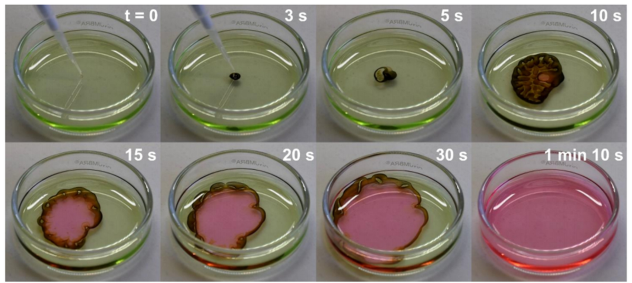
\includegraphics[scale=0.45]{figs/IodateIodine.png}
		\caption{\label{fig:iodateiodine}
		A drop of an iodine solution is placed in the an iodate solution. The reaction is 
		autocatalytic with respect to iodine, and a clear chemical front is observed where
		the iodate solution is ahead of the front and the rich iodine solution behind the front.
		Picture is from Panzarasa, \emph{Reaction Kinetics, Mechanisms and Catalysis}, 135:1349 (2022).
		}
	\end{center}
\end{figure}

The reaction rate can be modelled be applying \emph{mass action kinetics} such that
\begin{equation}
	\label{eq:rkcacb}
  r = k'c_Ac_B \, ,
\end{equation}
where $k'>0$ is the (second order) reaction rate coefficient, and $c_A$ and $c_B$ are the
concentration of $A$ and $B$, respectively. The rate of change for A is then
\begin{equation}
\label{eq:dcAdt}
  \frac{\d c_A}{\d t} = k'c_Ac_B \, .
\end{equation}
Let $c_0=c_A+c_B$ be the total concentration and assume this is a constant, then
\begin{equation}
  \frac{\d c_A}{\d t} = k'c_A(c_0 - c_A) \, .
\end{equation}
Allowing for diffusion and dividing with $c_0$ we have 
\begin{equation}
\frac{\partial c}{\partial t} = kc(1-c) + D \frac{\partial^2c}{\partial x^2}  \, ,
\end{equation}
where $c=c_A/c_0$ and $k=k'c_0$. This is the \emph{Fisher-Kolmogorov equation} or 
\emph{logistic growth with diffusion}. Notice that $c$ is bounded, $0 \leq c \leq 1$.

\begin{question}
	How did we arrive at Eq. (\ref{eq:dcAdt}) from Eq. (\ref{eq:rkcacb})?
\end{question}


Envision that we have a one dimensional system (i.e., a thin tube) 
composed of only reactive B molecules (and likely also an inert solvent). At time $t=0$
we introduce some A molecules at the left boundary, $x=0$. Encounters between A and B
molecules result in the autocatalytic production of A, leading to a local concentration
gradient and, hence, a flux where A molecules diffuse into rich B regions (positive $x$-direction),
where, again, A molecules are produced, and so forth. This, we may imagine,
leads to a propagating concentration front of A moving through the
system in the positive $x$-direction. Behind the front we have A molecules, and ahead of the front B
molecules; in the front zone both A and B molecules are present which react
according to (\ref{react:FK}). This is illustrated in Fig. \ref{fig:fronts}(a). 

One research question we now seek to answer is: \emph{If} the propagating front exists
and \emph{if} the speed is constant, how fast will the front propagate?

\begin{figure}
  \begin{center}
    \includegraphics[scale=0.4]{figs/FK-wavefront}
    \caption{\label{fig:fronts}
	  Propagating front in the standard (or fixed) coordinate system, (a), and in the
	  moving frame coordinate system, (b). The arrow in (a) indicates the direction of the 
	  front propagation (positive $x$-direction).
    }
  \end{center}
\end{figure}

Assume that (after a transient time) the front propagates with a
constant speed, $s$. We can then choose to shift the coordinate system 
with the front speed. In this moving frame the concentration profile is
independent of time. (Imagine you 'sit' on the front moving along with it, 
then you observe it being independent of time. This is not the case for an observer 
standing in a fixed coordinate system, where the front will pass her 
at some point in time.) Since the front propagates in the positive $x$-direction 
we define the moving frame coordinate by
\begin{equation}
  z = x - st \, .
\end{equation}
The concentration profile can now be written as being depended on $z$; 
$c(z)= c(z(x,t))=c(x,t)$. See Fig. \ref{fig:fronts} (b). Importantly, we must expect 
from our basic knowledge of dynamical systems that
\begin{equation}
  \lim_{z \rightarrow -\infty} c = 1  \ \text{and} \   \lim_{z \rightarrow
    \infty} c = 0 \, .
\end{equation}
This means that $c=1$ is an unstable fixed point and that $c=0$ is a stable fixed point. 

In our treatment here, we will require that for a front to exist there must be a $z_0$ such that
\begin{eqnarray}
	\left.\frac{\d c}{\d z} \right|_{z=z_0} \neq 0 
	\ \text{and} \ 
	\lim_{z \rightarrow \pm \infty} \frac{\d c}{\d z} = 0 \, .
\end{eqnarray}
To proceed we need to derive the dynamical equation for the concentration in the 
moving coordinate system. From the chain rule
\begin{equation}
  \frac{\partial c}{\partial t} = -s \frac{\d c}{\d z} \ \
  \text{and} \ \
  \frac{\partial^2 c}{\partial x^2} = \frac{\d^2 c}{\d z^2} \ . 
\end{equation}
Substitution into the Fisher-Kolmogorov equation gives 
\begin{equation}
  \label{eq:fkmvframe}
  D\frac{\d^2c}{\d z^2} + s\frac{\d c}{\d z} + kc(1-c) = 0 \, .
\end{equation}
Remember that $k>0$ since $k'>0$. 

This is an important result: As with the diffusion equation, we have managed to transform a 
partial differential equation into a problem of an ordinary differential equation. 
This is extremely helpful because we can now analyse this using
standard techniques. Also notice that $s$, which we hope to say something
about, enters the problem. 

In our analysis of the dynamics we start with a simple linear stability
analysis. First, we recast the second order differential equation into a system of first order equations 
\begin{eqnarray}
  \frac{\d c}{\d z} &=& v \nonumber \\
  D\frac{\d v}{\d z} &=& -sv - kc(1-c) \, .
\end{eqnarray}
where $v$ is an auxillary variable. The fixed points are 
\begin{equation}
  (c, v)=(0,0)  \ \text{and} \   (c, v)=(1,0) \, .
\end{equation}
From the previous discussion we expect that $(0,0)$ is stable and $(1,0)$ is
unstable, but sometimes our expectations will betray us, and we will now show this. 
The general Jacobian matrix is (please, check!)
\begin{equation}
  \mathbf{J} =
  \begin{bmatrix}
    0 & 1 \\
    k/D(c/2-1) & -s/D
    \end{bmatrix} \, .
\end{equation}
For the fixed point (1,0) we have the eigenvalues
\begin{equation}
  \lambda_{1,2}=-\frac{1}{2}\left(
    \frac{s}{D} \pm \sqrt{\left(\frac{s}{D}\right)^2 + \frac{4k}{D}} 
  \right) \, .
\end{equation}
Since $k>0$ and $D>0$, the sum under the square root is positive and the square root term is 
larger than $s/D$. This means that the eigenvalues are real, one being negative and one positive.
The point (1,0) is then an unstable saddle point. 

For the fixed point (0,0) we have the eigenvalues
\begin{equation}
  \lambda_{1,2}=-\frac{1}{2}\left(
    \frac{s}{D} \pm \sqrt{\left(\frac{s}{D}\right)^2 - \frac{4k}{D}} 
  \right) \, .
\end{equation}
The three possible scenarios are 
\begin{enumerate}
	\item{
			If $(s/D)^2>4k/D$, then the sum under the square root is positive and  
			$\left[\left(\frac{s}{D}\right)^2 - \frac{4k}{D}\right]^{1/2} < s/D$, that is, the eigenvalues are 
			both real and negative; the fixed point is a stable node. 
		}
	\item {
			If $(s/D)^2=4k/D$ we have repeated eigenvalues $\lambda_{1,2}=-2s/D$ and the 
			fixed point is a stable node.
		}
	\item {
			If $(s/D)^2 < 4k/D$ the fixed point has two complex conjugated eigenvalues with negative 
			real parts, that is, the fixed point is a stable spiral.
		}
\end{enumerate}
The last scenario is problematic when we interpret the function $c$ as being a normalized concentration since we then 
require $c \geq 0$. Recall,  $c(z)=c(x,t)=c_A/c_0 \geq 0$. If (0,0) is a stable spiral the 
phase plane trajectories will spiral around the origin (0,0) and $c$ will take negative values. Therefore, the eigenvalues 
cannot be complex, implying that only scenario 1 and 2 are useful. This in turn defines a minimum allowed speed, because 
\begin{equation}
\left(\frac{s}{D}\right)^2 \geq \frac{4k}{D} \ \Rightarrow s \geq 2\sqrt{kD} = s_\text{min}
\, .
\end{equation}
In Fig. (\ref{fig:minspeed}) the trajectories are shown for $s<s_\text{min}$ (the stable spiral case) 
and $s=s_\text{min}$ (the stable node case). 

\textit{Important} From the linear stability analysis we have only derived a minimum allowed
front propagation speed, not the actual speed the front takes. 
This is, furthermore, under the assumption that the front exists and propagates with constant speed. 
To investigate the system further we will rely on numerical analysis, see Exploration \ref{exploration:fisherKol}. 

\begin{figure}
\begin{center}
\includegraphics[scale=.4]{figs/minspeed}
\caption{\label{fig:minspeed} Two phase plane trajectories starting close to
	  the unstable saddle point (1,0). The  
	two examples are when $s = s_\text{min}$ and when $s < s_\text{min}$.
}
\end{center}
\end{figure}

We can do a bit more. Again, we will assume that the front exists and that it propagates with constant speed. 
Now, Eq. (\ref{eq:fkmvframe}) is a non-linear problem, which we cannot solve in general. However, we can find an 
approximate solution using a perturbation method. To this end, we identify a small perturbation parameter 
$\epsilon = 1/s^2$, that is, we focus our analysis on the limit of large front speeds. 
The choice of perturbation parameter is clear when we perform a second coordinate transformation  
\begin{equation} 
\xi = k z \sqrt{\epsilon} \, .
\end{equation}
From the chain rule we have the following identities
\begin{eqnarray}
	\frac{\d c}{\d z} = k\sqrt{\epsilon} \frac{\d c}{\d \xi} \ \ \text{and} \ \  
	\frac{\d^2 c}{\d z^2} = k^2 \epsilon \frac{\d c^2}{\d \xi^2} \, .
\end{eqnarray}
Substituting into Eq. (\ref{eq:fkmvframe}), we get
\begin{equation}
	\label{eq:fkinz}
\epsilon k D\frac{\d^2c}{\d \xi^2} + \frac{\d c}{\d \xi} + c(1-c) = 0 \, .
\end{equation}
This is a singular perturbation problem, since the case
$\epsilon=0$ yields a first order differential equation, which in general is
qualitatively different from the original differential equation. We boldly attempt to continue using the 
(naive) outer solution which we introduced for regular perturbation problems. 

We substitute the Poincar\'{e} expansion 
\begin{eqnarray}
	c(\xi) \sim \sum_{n=0}^N \epsilon^n c_n(\xi)
\end{eqnarray}
into Eq. (\ref{eq:fkinz}) and collect term wise. To zero'th order we obtain
\begin{equation}
\frac{\d c_0}{\d \xi} + c_0(1-c_0)=0 \, .
\end{equation}
This is a first order equation and, also, note it does not contain the diffusion
coefficient. This implies that we look at the effect of the reaction only, but
under the assumption that the front actually exists, hence, the diffusion process is 
implicitly included. Separation of variables gives
\begin{equation}
\frac{\d c_0}{c_0(1-c_0)} = \d \xi \, .
\end{equation}
\begin{wrapfigure}{R}{0.35\textwidth}
	\centering
	\includegraphics[width=0.3\textwidth]{figs/fku0.eps}
%	\caption{\label{fig:bacteriaindish} A figure.}
\end{wrapfigure}
\paragraph{}
\vspace*{-\parskip}
The fraction on the left-hand side can be written as
\begin{eqnarray}
	\frac{1}{c_0(1-c_0)} = \frac{1}{c_0} + \frac{1}{1-c_0} \, ,
\end{eqnarray}
and integration along some re-arrangement gives
\begin{equation}
	c_0 = \frac{1}{1+Ke^{\xi}} \, .
\end{equation}
We choose the IC $c_0(0)=1/2$ giving $K=1$ and therefore
\begin{equation}
c_0 = \frac{1}{1+e^{\xi}} = \frac{1}{1+e^{kz/s}} \, .
\end{equation}
This choice of IC is not unique; different choices will just shift the 
concentration profile in $\xi$-direction. If $s=s_\text{min}$ we get
\begin{equation}
\label{eq:u0fk} 
c_0 = \frac{1}{1+e^{\sqrt{k/(4D)}z}} \, .
\end{equation}
We continue the analysis in the exercises.

The idea of propagating fronts is used to model different systems. Let us see a two-species 
predator-prey example. 
\begin{example}\label{example:multifront}
	This example is from Murray, \textit{Mathematical Biology}; I will leave out 
	quite a few details and recommend that you to following along with pen and paper. 

	We consider predator movement from highly
	populated region of predators into low populated regions. The latter region is
	rich on prey due to the low predator concentration. This version of the model
	assumes that the prey does not perform any migration. Let
	$0 \leq c_1 \leq 1$ be the dimensionless prey concentration and
	$0 \leq c_2 \leq 1$ the dimensionless predator concentration. The model in 
	dimensionless form reads
	\begin{equation}
		\label{eq:pp0}
		\frac{\partial c_1}{\partial t} = c_1(1-c_1-c_2) \ ,
		\ \frac{\partial c_2}{\partial t} =
		ac_2(c_1-b) + \frac{\partial^2 c_2}{\partial x^2} \, ,
	\end{equation}
	where the model parameters follow that $a,b > 0$. 

	We assume that there exists a front and that the front speed is
	constant. We may once more ask the question ``If the front exists, what is the minimum allowed 
	propagation	speed?''. We approach the problem exactly as we did for the Fisher-Kolmogorov
	front, but, just for fun, in this example we let the front propagate from
	right to left (i.e, negative $x$-direction). This means that the moving frame coordinate is given by
	\begin{equation}
	z = x + st \, .
	\end{equation}
	Let $c_1(z)=c_1(x,t)$ and $c_2(z)=c_2(x,t)$. Then in the co-moving frame we have
	the dynamics
	\begin{eqnarray}
		s\frac{\d c_1}{\d z} &=& c_1(1-c_1-c_2) \\ 
		s\frac{\d c_2}{\d z} &=& ac_2(c_1-b) +\frac{\d^2c_2}{\d z^2} 
	\end{eqnarray}
	from which we can form a system of first order differential equations 
	\begin{eqnarray}
	\frac{\d c_1}{\d z}&=& \frac{c_1}{s}(1-c_1-c_2) \nonumber \\
	\frac{\d c_2}{\d z} &=& w  \label{eq:multifrontord}\\
	\frac{\d w}{\d z} &=& sw - ac_2(c_1-b)  \nonumber
	\end{eqnarray}
	Again, $w$ simply acts as an auxillary variables. The fixed points for this are 
	\begin{eqnarray}
		\text{unstable point}:  && (c_1,c_2,w)=(0,0,0) \nonumber \\
		\text{unstable point}: && (c_1,c_2, w)=(1,0,0) \nonumber \\
		\text{stable point}:  && (c_1,c_2,w)=(b,1-b,0) \nonumber 
	\end{eqnarray}
	The first fixed point is simply the trivial case, and is not interesting here. 
	The two other points are more informative:	As $z \rightarrow - \infty$ we approach the unstable fixed point (1,0,0), 
	that is, there is only prey ahead of the front. As $z \rightarrow \infty$ we approach the stable fixed 
	point $(b, 1-b, 0)$, this is the co-existence state between the prey and predator, having 
	concentrations $b$ and $1-b$, respectively. See illustration in Fig. \ref{fig:pp}.
	\begin{figure}
	\begin{center}
	  \includegraphics[scale=0.3]{figs/twospecies.eps}
	\end{center}
	\caption{\label{fig:pp} Illustration of the propagating front system in
		Example \ref{example:multifront}. Front propagation in the fixed frame is 
		indicated by the arrow. $b=2/3$}
	\end{figure}

	We demand that the concentrations are positive and bounded so $0 \leq c_1,c_2 \leq 1$. 
	We can then attempt the	same analysis as we did for the Fisher-Kolmogorov system, 
	but this time for the unstable fixed point (1,0,0). The Jacobian here reads 
	\begin{equation}
	\mathbf{J}(1,0,0) =
	\begin{bmatrix}
	  -1/s & -1/s & 0 \\
	  0 & 0 &1 \\
	  0 & a(b-1) & s
	\end{bmatrix}
	\end{equation}
	giving the three eigenvalues
	\begin{equation}
		\lambda_1 = -\frac{1}{s} \ \ \lambda_{2,3}=\frac{1}{2} \left(
		s \pm \sqrt{s^2 + 4a(b-1) }	\right)
	\end{equation}
	As we seek real eigenvalues, the minimum allowed speed is given by
	$s_\text{min} = 2\sqrt{a(b-1)}$.
\end{example}

\begin{question}
How can we interpret the reaction terms in Eq. (\ref{eq:pp0}) in context of a
predator-prey system? What is the biological interpretation of the parameters
$a$ and $b$?
\end{question}

\begin{exerciseregion}

	\begin{exercise}
		Perform a perturbation analysis of the Fisher-Kolmogorov front up to first
		order in $\epsilon$; you can express $c_1$ in terms of $c_0$. Hint: 
		(i) First, show that $1-2c_0=-c{''}_0/c{'}_0$. (ii) Then show that equation for the 
		first order term is
		\[
			\frac{\d c_1}{\d \xi} - \frac{c{''}_0}{c'_0}c_1 = -kD \frac{\d^2c_0}{\d \xi^2} \, .
		\]
		(iii) Solve this using the general identity from calculus
		\[
			\int \frac{f'(x)}{f(x)} \, \d x = \ln|f(x)| \, .
		\]
		(iv) Finally, use the intial value $u'_0(0)=1/4$ to find the particular solution.
	\end{exercise}

	\begin{exercise} \label{ex:checku0}
		Compare the zero'th order perturbation result, Eq. (\ref{eq:u0fk}), with
		numerical results for different front speeds. 
	\end{exercise}

	\begin{exercise}	
		Recall, our requirements for a front to exist. Can the linear problem
		\begin{eqnarray}
			\frac{\partial c}{\partial t}= c + \frac{\partial^2c}{\partial x^2}
		\end{eqnarray}
		feature a front? 
	\end{exercise}
	
	\begin{exercise}
		Through linear analysis of Eq. (\ref{eq:multifrontord}), show that the two-species 
		predator-prey model can feature (fascinating) oscillatory concentrations in the 
		front zone for certain choice of parameters.
	\end{exercise}

	\begin{exercise}
		In Example \ref{example:multifront}	the predator featured mobility. Will the model 
		support a propagating front if the predator is immobile, but the prey is mobile? 
		Model the mobility with a simple Fickian law.
	\end{exercise}

	\begin{exploration}
		\label{exploration:fisherKol}
		One main result from our study of the Fisher-Kolmogorov front is that
		$s > s_\text{min} = 2\sqrt{kD}$. As stated in the text, we do not know
		\emph{if} such front exists, and if so \emph{what} $s$ actually is. (We only
		know the minimum speed allowed.) Perform a numerical exploration of the
		system, and confirm whether the front exists (under different ICs). If so
		determine the stable front speed. [Note: Carefully explore the convergence of
		the wave speed.]
	\end{exploration}


	\begin{exploration}
	  The spread of dominant genes is modelled through an extended 
	  Fisher-Kolmogorov wavefront
	  \begin{equation}
		\label{eq:efk}
		\frac{\partial N}{\partial t} = k(N_0-N)N - N + D
		\frac{\partial^2N}{\partial x^2} \, .
	  \end{equation}
	  $N=N(x,t) \geq 0$ represents the dominant gene concentration, $k, N_0$, and
	  $D$ are the rate constant, total gene pool, and diffusion coefficient,
	  respectively. We let $x > 0$ and $t \geq 0$.

	  We assume that Equation (\ref{eq:efk}) allows for a
	  propagating wave with constant speed $s$. 
	  \begin{enumerate}
	  \item Perform a coordinate transformation using $z=x-st$ such that the
		wave is fixed in this coordinate system.
	  \item Show that $N \geq 0$ implies $kN_0 \geq 1$ if the wave front
		exists. What is the constant gene concentration behind the front?
	  \item Show that the minimum allowed speed is 
		$s_{\text{min}}=2\sqrt{D(kN_0-1)}$ if the front exists.
	  \item Perform numerical simulations confirming the results
		above. Describe what happens when $k=1$ $D=1$ and $N_0=0.5$
		(ignoring coefficient units). Clearly state your choice of boundary
		conditions.
	  \end{enumerate}
	\end{exploration}
\end{exerciseregion}


\section{Turing structures}
Recall Example \ref{example:turing}; in this section we will explore 
how these \emph{diffusion driven spatial structures} emerge in reaction-diffusion systems. 
At first thought, the existence of apparently spontaneously formed
structures contradict our intuition about diffusion processes which tend to reduce and eventually remove the gradients.  
However, for multi-variable systems and for certain types of reactions  
structures emerge and they can even be stable forming static structures with permanent  
spatial concentration gradients. The structures were first found theoretically by 
\emph{Alan Turing}\footnote{Whom, by the way, is also famous for inventing the 
Turing machine and cracking the Enigma code during the second world war.} in the early 1950s, 
which is why they also bare his name. 

We will here explore the Turing structures through the \emph{FitzHugh-Nagumo (FHN) model} 
used to study different excitable systems. For example, 
it is the standard model for a neuron electrical signal (also called neuron firing) caused 
by voltage build-up and release. A simple version of the model is 
in the homogeneous case (where we can ignore diffusion)
\begin{eqnarray}
	\label{eq:fhn1}
	\frac{\d c_1}{\d t} &=& c_1 - c_1^3 - c_2 + \alpha = r_1\\
	\label{eq:fhn2}
	\frac{\d c_2}{\d t} &=& \beta(c_1 - c_2) = r_2
\end{eqnarray}
where $c_1$ is the voltage and $c_2$ acts as a coarse grained variable that describes the 
coupling between the voltage and other relevant cell mechanisms. Notice, the function definitions 
of $r_1$ and $r_2$ on the right-hand; they will be used below. 
The model parameters fulfill $\alpha, \beta > 0$. For now, we will not go into a 
more detailed bio-physical interpretation of the model, and right away
start the mathematical analysis. 

t is easy to verify that there exists a single fixed point, namely, 
\begin{equation}
	(\alpha^{1/3}, \alpha^{1/3}) = (a, b)\, .
\end{equation}
Notice that we will use the symbols $a$ and $b$ for the fixed point coordinates; this is just 
to ease and clarify the reading a bit. It is worth to recapture some of the details in the standard 
linear analysis: We first linearise the dynamical equations in a neighbourhood 
around the fixed point $(a,b)$. For $r_1$ we have
\begin{eqnarray}
	r_1 &=& r_1(a,b) + \frac{\partial r_1}{\partial c_1}(c_1-a) + \frac{\partial r_1}{\partial c_2}(c_2-b) + \ldots \\
				 &=&	(1-3a^2) u - v + \dots
\end{eqnarray}
where $u$ and $v$ describe the deviation of $c_1$ and $c_2$ to the fixed point
\begin{equation}
	u = c_1 - a \ \ \text{and} \ \ v = c_2 - b \, .
\end{equation}
For $r_2$ we have 
\begin{equation}
	r_2 = \beta u - \beta v + \ldots
\end{equation}
We can now readily write the Jacobian in the fixed point 
\begin{equation}
\matrx{J} = 
	\begin{bmatrix}
    1-3\alpha^{2/3} & -1 \\
    \beta & -\beta
 \end{bmatrix} \, ,
\end{equation}
and the eigenvalues are found from the characteristic polynomial
\begin{equation}
	\lambda^2 + (\beta-1+3\alpha^{2/3})\lambda + 3\beta\alpha^{2/3} = 0 \, .
\end{equation}
Without loosing the main conclusions we choose $\alpha$ such that $\alpha^{2/3}=1/10$; 
in this case the eigenvalues are 
\begin{equation}
	\lambda_{1,2} = \frac{1}{2}\left(
	\frac{7}{10}-\beta \pm \sqrt{\beta^2-13\beta/5+49/100} 
	\right) \, .
\end{equation}
We see that the eigenvalues are complex (and conjugate) 
whenever $\beta^2-13\beta/5+49/100<0$ implying that in the interval
\begin{eqnarray}
	\frac{1}{10}\left(13 - \sqrt{120}\right) < \beta <  \frac{1}{10}\left(13 + \sqrt{120}\right) 
\end{eqnarray}
the system features oscillatory behaviour. 

In this interval the real part of the eigenvalues also
changes sign indicating that a bifurcation occurs ($\beta$ being the bifurcation parameter). 
A bit more formally, we expect a bifurcation at $\beta=7/10$, where 
$\text{Re}(\lambda_{1,2})=0$ and where 
\begin{eqnarray}
	\frac{\d\text{Re}(\lambda_{1,2})}{\d \beta} = -1/2 \neq 0 \, .
\end{eqnarray}
This last property is \emph{the transversal condition} which ensures 
that the eigenvalue real part, in fact, changes sign. Thus, we have 
\begin{description}
	\item[$(13 - \sqrt{120})/10 < \beta < 7/10$]{The fixed point is an unstable spiral point}
	\item[$\beta = 7/10$]{The fixed point is non-hyperbolic (the stability is unknown from the linear analysis)}
	\item[$7/10 <\beta < (13 + \sqrt{120})/10$]{The fixed point is a stable spiral.}
\end{description}
This indicates a \emph{Hopf bifurcation} at $\beta = 7/10$: 
(i) For $\beta < 7/10$ the solution converges to a stable \emph{limit cycle}, 
i.e, the system has sustained oscillations (with respect to time) 
below the bifurcation parameter value. See Fig. \ref{fig:fhnbif}. 
(ii) For $\beta > 7/10$ the oscillations are dampened 
and the system relaxes to the stable fixed point. 
Both the condition $\text{Re}(\lambda_{1,2})=0$ and the transversal 
condition are necessary, but not sufficient, conditions for a Hopf bifurcation. 
\begin{figure}
  \begin{center}
    \includegraphics[scale=.45]{figs/fhnPhasePortrait.eps}
    \caption{
    \label{fig:fhnbif} Phase plane trajectories for the FHN model system. 
	  Left: $\beta < 7/10$. Right: $\beta>7/10$.
		Fixed point illustrated by the filled circle. 
		Trajectories are obtained from numerical solutions.
    }
  \end{center}
\end{figure}


We now include diffusion for both $c_1$ and $c_2$ and show that if the diffusion coefficients 
are different, $D_1 \neq D_2$, the system can be unstable in the parameter interval 
$7/10 <\beta < (13 + \sqrt{120})/10$ and $\alpha^{2/3} = 1/10$, 
that is, in the interval where the homogeneous case is stable.  

Again we perform a linear stability analysis, but this time for the full RD-equation. 
First we note that 
\begin{equation}
	\frac{\partial c_1}{\partial t} = \frac{\partial u}{\partial t} \ \ \text{and} \ \ 
	\frac{\partial^2 c_1}{\partial x^2} = \frac{\partial^2 u}{\partial x^2}
\end{equation}
and so forth for the derivatives of $c_2$ and $v$. Then we can write the linearized 
RD-equations in terms of $u$ and $v$, i.e, in terms of the deviation from the homogeneous fixed point
\begin{eqnarray}
	\label{eq:fhnlin1}
	\frac{\partial u}{\partial t} &=& (1-3\alpha^{2/3})u - v + D_1 \frac{\partial^2 u}{\partial x^2}\\
	\label{eq:fhnlin2}
	\frac{\partial v}{\partial t} &=& \beta(u-v) + D_2 \frac{\partial^2 v}{\partial x^2}
\end{eqnarray}
with $D_1$ and $D_2$ being the usual diffusion coefficients. The boundaries we apply here are the zero Neumann BCs 
\begin{equation}
	\left.\frac{\partial u}{\partial x}\right|_{x=0} = \left.\frac{\partial u}{\partial x}\right|_{x=L} = \left.\frac{\partial v}{\partial x}\right|_{x=0} = \left.\frac{\partial v}{\partial x}\right|_{x=L} = 0 \, .
\end{equation}
The initial condition is such that the spatial average of $u$ and $v$ are zero, that is, with some $u$ and $v$ are randomly distributed around the
point $(a,b)$ with sufficiently small amblitude. 

From our earlier experience with the linear RD-equation under Neumann BCs 
we expect that the solutions for $u$ and $v$ are cosine Fourier series, that is,
\begin{equation}
\label{eq:turingguess}
	u(x,t) = \sum_{n=1}^\infty u_n e^{\lambda_n t}\cos\left(\frac{n\pi}{L} \, x\right) \ \ \text{and} 
	\ \ v(x,t) = \sum_{n=1}^\infty v_n e^{\lambda_n t}\cos\left(\frac{n\pi}{L} \, x\right) \, . 
\end{equation}
We do not know $\lambda_n$, that is, in our proposition the temporal dynamics is still undetermined. 
Now, the solutions must of course fulfill the two linearized equations. Thus, 
substituting the guess, Eq. (\ref{eq:turingguess}), into Eq. (\ref{eq:fhnlin1}) and differentiating we get
for each term, $n$, we have
\begin{eqnarray}
	\lambda_n u_n e^{\lambda_n t} \cos\left(\frac{n\pi}{L} \, x\right) 
	&=& \frac{7}{10}u_n e^{\lambda_n t} \cos\left(\frac{n\pi}{L} \, x\right)  \nonumber \\
	&-& v_n e^{\lambda_n t} \cos\left(\frac{n\pi}{L} \, x\right) 
	- D_1 u_n \left(\frac{n\pi}{L}\right)^2 e^{\lambda_n t} \cos\left(\frac{n\pi}{L} \, x\right)
	\nonumber \\
\end{eqnarray}
using the value $\alpha^{2/3}=1/10$. The exponential terms cancels, and if we rearrange we obtain
\begin{equation}
	\left(
		\lambda_n u_n -\frac{7}{10} u_n + v_n + \left(\frac{n\pi}{L}\right)^2 u_n D_1
	\right) \cos\left(\frac{n\pi}{L} \, x\right) = 0 \, . 
\end{equation}
Repeating this for Eq. (\ref{eq:fhnlin2}) we get the identity 
\begin{equation}
	\left( \lambda_n v_n - \beta u_n + \beta v_n + \left(\frac{n\pi}{L}\right)^2 v_n D_2
	\right) \cos\left(\frac{n\pi}{L} \, x\right) = 0 \, .
\end{equation}
We can combine these two equations and obtain a more convenient (and hopefully recognizable) form. 
First, let $\vec{W}_n = (u_n, v_n)^T$ and recall that the 
diffusion matrix is defined as
\begin{equation}
	\mathbf{D} =
	\begin{bmatrix}
	D_1 & 0 \\
	0 & D_2
	\end{bmatrix}
\end{equation}
then we have on matrix-vector form
\begin{equation}
	\left[
		\lambda_n \matrx{I} - \matrx{J} + \left(\frac{n\pi}{L}\right)^2 \, \matrx{D}
	\right] \cdot \vec{W}_n \cos\left(\frac{n\pi}{L} \, x\right) = \vec{0} \, .
\end{equation}
This, you may see, is an eigenvalue problem. As usual, we do not seek the trivial case 
$\vec{W}_n=\vec{0}$, as this leads to the trivial solutions for $u_n$ and $v_n$. 
A non-trivial solution exists if the matrix
\begin{equation}
	\left[
		\lambda_n \matrx{I} - \matrx{J} + \left(\frac{n\pi}{L}\right)^2 \, \matrx{D}
	\right]
\end{equation}
is rank deficient, that is, if there exists one or two $\lambda_n$ such that the determinant is zero
\begin{eqnarray}
\label{eq:turingeig}	
	\mbox{} & \left|
		\lambda_n \matrx{I} - \matrx{J} + \left(\frac{n\pi}{L}\right)^2 \, \matrx{D}
	\right| = 
	\left(
		\lambda_n - \frac{7}{10} +\left(\frac{n\pi}{L}\right)^2 D_1
	\right) 
\left(
	\lambda_n + \beta +\left(\frac{n\pi}{L}\right)^2 D_2
	\right) + \beta = 0  \, . \nonumber \\
\end{eqnarray}
Before solving this quadratic problem, we introduce the two auxiliary variables 
\begin{eqnarray}
	a_n = -\frac{7}{10} + k^2 D_1, \text{and} \  \
	b_n = \beta + k^2 D_2
\end{eqnarray}
where $k=n\pi/L$ is the wave vector. The solution can now be written as 
\begin{eqnarray}
	\lambda_{n,1,2} = \frac{1}{2}\left( 
		-(a_n+b_n) \pm \sqrt{(a_n+b_n)^2 - 4(\beta + a_nb_n)}
	\right) \, .
\end{eqnarray}
Notice that the eigenvalues are functions of $n, \beta, D_1$, and $D_2$. 

We can know investigate the dynamics for each Fourier term (or Fourier mode): 
If the real part of the eigenvalue is negative for a given mode
this mode is stable, whereas if the real part is positive the mode is unstable. As always, in case 
of zero real part (the non-hyperbolic case) we cannot conclude anything about the stability of 
the system. Figure \ref{fig:dispersion} shows the real part of the eigenvalues $\lambda_{n}$ 
as function of wave vector, which is equivalent to a plot of the real part of 
$\lambda_n$ versus $n$. This is the \emph{dispersion plot}, 
and the eigenvalue's dependency on $k$ is called a \emph{dispersion relation}. We have used 
$D_2 = 10D_1$ and $\beta=1$. 
\begin{figure}
	\begin{center}
    \includegraphics[scale=.3]{figs/dispersion}
    \caption{
		\label{fig:dispersion} Dispersion plot: Real part of the eigenvalues, $\lambda_{n}$ 
		as a function of $k=n\pi/L$. $D_2 = 10 D_1$, $\alpha = (1/10)^{3/2}$, and $\beta = 1$. 
	}
  \end{center}
\end{figure}
Some of the Fourier modes (indicated by the blue interval) are unstable, hence, the  
solution to the linearized system, Eq. (\ref{eq:turingguess}), grows exponential in time and the 
system is unstable. 

This is a linear analysis. The non-linear part of the system may eventually 
suppress this growth as $u$ and $v$ become sufficiently large and thus form a 
steady state structure. 

We can solve the non-linear RD-equation using the FTCS algorithm. We will do this using 
the same parameter values as in
Fig. \ref{fig:dispersion}. The voltage $c_1$ is plotted as function of $x$ for four different times 
in Fig. \ref{fig:turingfhn}. It is seen that the structure emerge from the homogeneous state reaching a 
final steady state. 
\begin{figure}
  \begin{center}
    \includegraphics[scale=.3]{figs/turingfhn}
    \caption{
		\label{fig:turingfhn} 
		FHN model voltage profiles as function of $x$ for four different times. 
		Black line is the condition. Red and green lines are 
		transient profiles, and blue is the final steady state profile. 
		Parameter values are the same as in Fig. \ref{fig:dispersion}.
    }
  \end{center}
\end{figure}
An important observation from the numerical simulations is that the (characteristic) period of the 
structure is given by
\begin{eqnarray}
	p = 2\pi/k_\text{max} \, .
\end{eqnarray}
$k_\text{max}$ is also shown in Fig. \ref{fig:dispersion}. This means that the Fourier mode with largest 
eigenvalue (real part) grows the fastest and dominates the final steady state. 
Again, this is all based on the linear analysis and not some thing we can conclude in general. 

We end this section by listing three necessary conditions for a system to feature 
diffusion-driven instabilities (or Turing structures). 

\begin{theorem}
	\label{th:turing}
	Consider a two species RD-equation with equilibrium point $(a,b)$ and Jacobian
	\begin{eqnarray}
		\mathbf{J}(a,b) = 
		\left[	\begin{matrix}
			a_{11} & a_{12} \\
			a_{21} & a_{22}
		\end{matrix}
		\right]
	\end{eqnarray}
	\emph{If} the system feature Turing structures then
	\begin{enumerate}
		\item $a_{11} a_{22} < 0 $
		\item $a_{12} a_{21} < 0 $
		\item $D_1 \neq D_2$.
	\end{enumerate}
	We will not proof this theorem.
\end{theorem}

\begin{exerciseregion}
	\begin{exercise}
		For the FitzHugh-Nagumo model use $D_1=1, \alpha=(1/10)^{3/2}, \beta=2$, and $L=200$. 
		Find the values for $D_2$ and corresponding wavenumbers $n$, where unstable Fourier modes emerges. 
		Predict the wavelength, and confirm your findings from numerical simulations of the RD-eq system.
	\end{exercise}
	\begin{exercise}
		Theorem \ref{th:turing} limits the possibilities of signs the Jacobian matrix elements can have. Illustrate 
		this by writing the Jacobian with the elements sign only. (This leads to two concepts, namely, 
		\emph{activator-inhibitor} and \emph{positive feedback}. 
	\end{exercise}
	\begin{exercise}
		Recall the Lotka-Volterra predator-prey model 
		\begin{eqnarray}
			\frac{\d c_1}{\d t} &=& c_1 - c_1c_2 \nonumber \\
			\frac{\d c_2}{\d t} &=& c_1c_2 - \alpha c_2
		\end{eqnarray}
		with $\alpha>0$ and $c_1,c_2 \geq 0$. 
		Does the corresponding RD-equation allow for diffusion-driven instabilities?
	\end{exercise}
	\begin{exploration}
		We consider the RD-equation system
		\begin{eqnarray}
			\frac{\partial c_1}{\partial t} = \frac{c_1^2}{c_2} - b c_1 + \frac{\partial^2 c_1}{\partial x^2} \\
			\frac{\partial c_2}{\partial t} = c_1^2 - c_2 + D \frac{\partial^2 c_2}{\partial x^2}
		\end{eqnarray}
		Determine the fixed point for $c_1, c_2 > 0$ in the homogeneous case. 
		Then determine critical value for $b$, where this fixed point is stable. 
		Now, choose $b=0.5$, and find the dispersion curve for different values of $D$; identify the range of 
		possible unstable Fourier modes on the curve. Based on this analysis, explore numerically 
		whether Turing structures 
		exists or not. (Inspired by Murray, \textit{Mathematical Biology}.) 
	\end{exploration}
	
\end{exerciseregion}




